\documentclass[10pt,a4paper,twocolumn]{article}
\newcommand{\runningtitle}{Reconstrucción barión-antibarión a 50 MeV}
\newcommand{\paperfooter}{Manuscrito de investigación | 9 de octubre de 2026}
\usepackage[utf8]{inputenc}
\usepackage[T1]{fontenc}
\usepackage{lmodern}
\usepackage[margin=17mm,top=18mm,bottom=19mm,columnsep=6.5mm]{geometry}
\usepackage{amsmath,amssymb,array,booktabs,graphicx,xcolor,microtype}
\usepackage[authoryear,round]{natbib}
\usepackage{caption,stfloats,fancyhdr,balance}
\usepackage{multicol}
\usepackage[unicode,colorlinks=true,linkcolor=navy,citecolor=navy,urlcolor=navy]{hyperref}
\definecolor{navy}{HTML}{173B56}
\setlength{\parindent}{1em}
\setlength{\parskip}{1pt}
\setlength{\emergencystretch}{1.7em}
\setlength{\intextsep}{9pt}
\setlength{\textfloatsep}{11pt}
\setlength{\dbltextfloatsep}{11pt}
\setcounter{topnumber}{3}
\setcounter{dbltopnumber}{2}
\renewcommand{\topfraction}{.92}
\renewcommand{\dbltopfraction}{.95}
\renewcommand{\textfraction}{.08}
\renewcommand{\floatpagefraction}{.82}
\renewcommand{\dblfloatpagefraction}{.82}
\captionsetup{font=small,labelfont=bf,labelsep=period,skip=5pt}
\pagestyle{fancy}
\fancyhf{}
\fancyhead[L]{\footnotesize\color{navy}\runningtitle}
\fancyhead[R]{\footnotesize Andrés Germán García}
\fancyfoot[L]{\footnotesize\paperfooter}
\fancyfoot[R]{\footnotesize\thepage}
\setlength{\headheight}{13pt}
\renewcommand{\headrulewidth}{.35pt}
\newcommand{\fB}{f^{(s)}_{B\bar B}}
\newcommand{\sB}{s_{B+\bar B}}
\newcommand{\stot}{s_{\mathrm{tot}}}
\newcommand{\shad}{s_{\mathrm{had}}}
\newcommand{\sL}{s_{\mathrm{light}}}
\newcommand{\YB}{Y_{\Delta B}}
\newcommand{\doi}[1]{\href{https://doi.org/#1}{doi:#1}}
\newcommand{\fulltitle}[3]{%
\twocolumn[%
\begin{center}
{\fontsize{18}{20.5}\selectfont\bfseries\color{navy}#1\par}
\vspace{8pt}
{\normalsize Andrés Germán García\par}
{\small #2\par}
\vspace{7pt}
{\small #3\par}
\end{center}
\vspace{6pt}
\begin{minipage}{\textwidth}
\textbf{\abstractlabel.} \abstracttext
\vspace{6pt}\par
\textbf{\keywordslabel:} \keywordstext
\end{minipage}
\vspace{15pt}
]%
}


\renewcommand{\figurename}{Figura}
\renewcommand{\tablename}{Tabla}
\renewcommand{\refname}{Referencias}
\newcommand{\abstractlabel}{Resumen}
\newcommand{\keywordslabel}{Palabras clave}
\newcommand{\abstracttext}{El objetivo fue comprobar si las masas de reposo, el espín y las cargas de las especies de partícula, combinados con la abundancia cosmológica actual, permiten reconstruir poblaciones de bariones y antibariones durante la época de aniquilación y contrastarlas con la literatura. Se utilizó un gas ideal de resonancias hadrónicas con inventarios PDG2014, PDG2020 y PDG2025 fijados, conservando sus masas. Se adoptó 50 MeV como referencia bibliográfica aproximada y se resolvió el potencial químico bariónico mediante el exceso observado por unidad de entropía, manteniendo $\mu_Q=\mu_S=0$. Se localizaron raíces, se verificaron sumas térmicas con integrales independientes y se examinó la unicidad del mapa neto. A 50 MeV, PDG2025 dio $2.7261\times10^{30}$ bariones y $2.7172\times10^{30}$ antibariones por cm$^3$, con exceso de $8.8765\times10^{27}$ cm$^{-3}$. El cociente antibariones/exceso fue 306.1147 y la participación nucleónica, 95.2176\%. El criterio de igualdad entre antibariones y exceso neto se alcanzó a 38.203739 MeV, que redondea al valor publicado de 38.2 MeV. Variar sólo $\eta$ dentro de su incertidumbre de entrada produjo 38.192814--38.214598 MeV. La comparación comóvil conservó el residuo y permitió relacionar los totales con una región de volumen actual explícito. La reconstrucción fue posible bajo temperatura, equilibrio y conservación declarados; el presente solo no identificó una historia única. La simplificación química dejó carga y extrañeza netas sin anular. Los resultados aportan una referencia reproducible de equilibrio, cuyo alcance histórico completo requiere balances químicos y evolución cinética adicionales.}
\newcommand{\keywordstext}{abundancia bariónica; aniquilación; equilibrio térmico; masa de reposo; reconstrucción retrospectiva; resonancias hadrónicas.}
\hypersetup{pdftitle={Reconstrucción del sector barión-antibarión a 50 MeV: masas de reposo y abundancias cosmológicas},pdfauthor={Andrés Germán García}}
\begin{document}
\fulltitle{Reconstrucción del sector barión-antibarión a 50 MeV:\\masas de reposo y abundancias cosmológicas}{Investigador independiente, México}{Reconstrucción de equilibrio y contraste con la literatura | 9 de octubre de 2026}
\section{Introducción}
La abundancia bariónica actual conserva información sobre el exceso de materia respecto de antimateria, pero reconstruir las cantidades que coexistieron durante la aniquilación exige establecer qué información adicional aporta un modelo térmico. Dos inventarios con igual diferencia entre bariones y antibariones pueden contener cantidades de pares muy distintas. Por ello, la pregunta retrospectiva debe distinguir el residuo observado de la población total inferida a una temperatura especificada.

La literatura ofrece referencias concretas para situar esa comparación. \citet{Satarov2013} describen abundancias de bariones y antibariones casi iguales por encima de aproximadamente 50 MeV y una disminución rápida de la proporción de antibariones al enfriarse el plasma por debajo de esa escala. \citet{Yang2022} estudian la ventana de 50 a 30 MeV y publican 38.2 MeV para el criterio $n_{\bar B}/(n_B-n_{\bar B})=1$. Estos hitos describen la evolución de las abundancias; 50 MeV no es una medición del primer evento de aniquilación y el segundo criterio no exige que los antibariones hayan desaparecido.

El gas de resonancias hadrónicas, HRG por sus siglas en inglés, permite calcular poblaciones de equilibrio a partir de masas de reposo, espín y cargas de las especies de partícula. Las listas de Thermal-FIST proporcionan un inventario documentado para ese cálculo \citep{Vovchenko2019,TFLists2026}. En este trabajo, las propiedades tabuladas constituyen las firmas utilizadas para identificar cada especie de partícula. No se analizaron señales espectrales originales de la época temprana. La abundancia cosmológica actual se incorporó como restricción externa del número bariónico neto.

El objetivo fue comprobar si esas propiedades, combinadas con la abundancia actual y una temperatura fundamentada en la literatura, permiten inferir por separado las poblaciones tempranas de bariones y antibariones, cuantificar su relación con el residuo y contrastar el resultado con lo publicado. Se evaluó también si el presente determina una reconstrucción histórica única. El análisis se centró en 50 MeV y en la localización del cruce publicado, conservando las masas del inventario HRG y declarando las condiciones que hacen posible la inferencia.

\section{Métodos}
\subsection{Diseño, datos y alcance del inventario}
Se realizó una reconstrucción matemática de estados de equilibrio. Se adoptó 50 MeV como referencia bibliográfica aproximada y se evaluaron puntos entre 37 y 50 MeV para localizar el cruce de abundancias. Los puntos intermedios fueron evaluaciones numéricas, sin asignarles nuevas épocas físicas. Se utilizaron unidades naturales, $\hbar=c=k_B=1$, con masas y temperaturas en GeV.

Se leyeron las listas PDG2014, PDG2020 y PDG2025 del repositorio Thermal-FIST, fijadas en la revisión \texttt{4086191e9522} \citep{TFLists2026}. El suplemento contiene el identificador completo, archivos originales, licencia y huellas SHA-256. Se conservaron las masas nominales y degeneraciones de espín; se excluyeron líneas comentadas y entradas de degeneración cero. Cada estado de carga se contó según su entrada, y las antipartículas se incluyeron por separado cuando correspondía. Todas las entradas bariónicas activas tenían $|B_i|=1$.

\begin{table}[t]
\centering\small
\caption{Dimensiones de los inventarios utilizados. Las especies activas incluyen antipartículas; $B+\bar B$ cuenta las entradas bariónicas activas.}
\label{tab:inventory}
\setlength{\tabcolsep}{4pt}
\begin{tabular}{lrrr}\toprule
Lista & Filas & Especies activas & $B+\bar B$\\\midrule
PDG2014 & 219 & 387 & 260\\
PDG2020 & 242 & 433 & 298\\
PDG2025 & 248 & 443 & 292\\
\bottomrule\end{tabular}
\end{table}

Las listas abarcan el sector de quarks $u,d,s$; no se agregaron núcleos ni listas de otros sectores de quarks. Se adoptó un HRG ideal, con masas fijas, anchos de resonancia nulos y temperatura común. No se incorporaron correcciones de volumen excluido ni una evolución de reacciones. Se mantuvieron $\mu_Q=\mu_S=0$ y se resolvió $\mu_B$. Esta simplificación no impone neutralidad eléctrica ni extrañeza neta nula; tampoco se resolvieron potenciales químicos leptónicos que compensaran la carga.

\subsection{Densidades y entropía por especie de partícula}
Para cada especie de partícula masiva se calculó
\begin{equation}
n_i=\frac{g_i m_i^2T}{2\pi^2}
\sum_{k=1}^{K_{\max}}\frac{c_{i,k}}{k}
K_2(kx_i)e^{k\alpha_i},\label{eq:number}
\end{equation}
con $x_i=m_i/T$, $\alpha_i=\mu_i/T$ y $\mu_i=B_i\mu_B$. Aquí $g_i=2J_i+1$; $c_{i,k}=1$ para bosones y $c_{i,k}=(-1)^{k+1}$ para fermiones. $K_\nu$ denota la función de Bessel modificada de segunda clase. Estas expresiones implementan las distribuciones de Bose-Einstein y Fermi-Dirac; no describen una prueba estadística sobre mediciones.

La entropía se obtuvo con el mismo potencial químico:
\begin{align}
s_i&=\frac{g_i m_i^2T}{2\pi^2}
\sum_{k=1}^{K_{\max}}c_{i,k}e^{k\alpha_i}\bigg[
\frac{4K_2(kx_i)}{k^2}\nonumber\\
&\qquad+\frac{x_iK_1(kx_i)}{k}
-\frac{\alpha_iK_2(kx_i)}{k}\bigg].\label{eq:entropy}
\end{align}
Se usaron 96 términos en las sumas y 192 en el control de convergencia. Los mesones tuvieron $\mu_i=0$. La entropía total incluyó hadrones, fotones, electrones y positrones, muones y antimuones, y tres sabores de neutrinos y antineutrinos:
\begin{equation}
s_{\rm tot}=s_{\rm had}+s_\gamma+s_{e^\pm}
+s_{\mu^\pm}+s_{\nu\bar\nu}.\label{eq:stotal}
\end{equation}
Fotones, electrones y neutrinos se trataron como componentes sin masa, con degeneraciones conjuntas 2, 4 y 6. Se utilizó $s_{\rm rel}=(2\pi^2/45)gT^3$, multiplicado por $7/8$ para fermiones. Los muones se calcularon como partículas masivas con $m_\mu=0.1056583755$ GeV y degeneración conjunta 4 \citep{PDG2025}. Se fijaron a cero los potenciales químicos del sector ligero.

Se definieron $n_\Sigma=n_B+n_{\bar B}$ y $\Delta n_B=n_B-n_{\bar B}$, junto con $Y_i=n_i/s_{\rm tot}$. En unidades físicas, el denominador del rendimiento es $s_{\rm tot}/k_B$, expresado en las mismas unidades de volumen que $n_i$. Las densidades naturales se convirtieron a cm$^{-3}$ con $\hbar c=1.973269804\times10^{-14}$ GeV cm \citep{Robinson2025}. La conversión de temperatura utilizó $k_B=8.617333262\times10^{-5}$ eV K$^{-1}$.

\subsection{Restricción cosmológica y solución inversa}
Se adoptó $\eta=(6.12\pm0.04)\times10^{-10}$ como entrada externa CMB, compilada por \citet{Fields2025}. La conservación adiabática de entropía y del número bariónico neto dio
\begin{equation}
\frac{\Delta n_B(T,\alpha)}{s_{\rm tot}(T,\alpha)}
=Y_{\Delta B}^{\rm ref}=\frac{\eta}{7.04},
\quad\alpha=\frac{\mu_B}{T}.\label{eq:inverse}
\end{equation}
El factor 7.04 convierte la abundancia por fotón del presente en abundancia por entropía, bajo la aproximación estándar posterior a la aniquilación $e^+e^-$. No se impuso $s(T)/n_\gamma(T)=7.04$ al plasma de 50 MeV.

Para evitar la pérdida de precisión por restar poblaciones casi iguales, se definió $a_{i,k}=g_i m_i^2T c_{i,k}K_2(kx_i)/(2\pi^2k)$ para las entradas $B_i=+1$ y se evaluó
\begin{align}
n_\Sigma&=2\sum_{i,k}a_{i,k}\cosh(k\alpha),\nonumber\\
\Delta n_B&=2\sum_{i,k}a_{i,k}\sinh(k\alpha).\label{eq:stable}
\end{align}
La entropía del par se sumó de forma equivalente mediante funciones hiperbólicas. Se resolvió la ecuación~\eqref{eq:inverse} con el método de Brent, en $0\leq\alpha\leq1$, con tolerancias absoluta $10^{-18}$ y relativa $10^{-13}$. Se recuperaron $n_B=(n_\Sigma+\Delta n_B)/2$ y $n_{\bar B}=(n_\Sigma-\Delta n_B)/2$.

Para contrastar el mismo criterio de \citet{Yang2022} se definió
\begin{equation}
R(T)=\frac{n_{\bar B}}{\Delta n_B}
=\frac{Y_{\bar B}}{Y_{\Delta B}}.\label{eq:ratio}
\end{equation}
Un segundo cálculo de raíz localizó $R(T_\times)=1$ dentro de 37--40 MeV, con tolerancias absoluta $10^{-10}$ MeV y relativa $10^{-13}$. Este intervalo fue un encuadre numérico del cruce, no una temperatura inicial ajustada para producir concordancia. Se repitió la solución con los tres catálogos y con los extremos $\eta=6.08$ y $6.16\times10^{-10}$, variando sólo esa entrada.

\subsection{Comparación con el presente y prueba de unicidad}
Con $T_{\gamma0}=2.7255\pm0.0006$ K, redondeado de \citet{Fixsen2009}, se calcularon
\begin{align}
n_{\gamma0}&=\frac{2\zeta(3)}{\pi^2}
\left(\frac{k_BT_{\gamma0}}{\hbar c}\right)^3,\nonumber\\
s_0/k_B&\simeq7.04n_{\gamma0},\qquad
n_{b0}=\eta n_{\gamma0}.\label{eq:present}
\end{align}
Para comparar cantidades en la misma región comóvil se utilizó $s(T)V(T)=s_0V_0$ y, por tanto,
\begin{equation}
N_i(T)=Y_i(T)(s_0/k_B)V_0.\label{eq:comoving}
\end{equation}
Se eligió $V_0=1$ m$^3$ como normalización explícita; los números resultantes son cantidades medias y pueden ser fraccionarios. No se adoptó un volumen para todo el Universo.

La composición primordial equivalente a la densidad media actual se convirtió usando $Y_p=0.245\pm0.003$ y $(D/H)_{\rm P}=(2.508\pm0.029)\times10^{-5}$ \citep{Fields2025}: $n_{H0}^{\rm prim}\simeq(1-Y_p)n_{b0}$, $n_{{}^4He,0}^{\rm prim}\simeq Y_p n_{b0}/4$ y $n_{D0}^{\rm prim}\simeq(D/H)_{\rm P}n_{H0}^{\rm prim}$. Se despreciaron las correcciones de núcleos traza al balance H/He, las correcciones de enlace, el procesamiento estelar y la ionización. Se propagaron incertidumbres a primer orden suponiendo entradas independientes; las salidas comparten entradas y están correlacionadas.

La unicidad se examinó con el mapa $(Y_B,Y_{\bar B})\mapsto Y_B-Y_{\bar B}$. Su matriz $[1,-1]$ tiene rango uno y dirección nula $(1,1)$. Esta propiedad identifica la información que falta en el residuo, sin proponer historias cinéticas adicionales.

\subsection{Verificación y tratamiento de incertidumbres}
Los 24 controles registrados compararon 96 y 192 términos, comprobaron el cierre de la restricción cosmológica y contrastaron número, exceso y entropía de protones y neutrones con integrales independientes a potencial químico finito. Se verificaron las huellas de los catálogos y se exportaron resultados agregados y por especie de partícula. Las tablas y figuras se generaron directamente de esos archivos.

No se hicieron pruebas de hipótesis, ajustes a observaciones nuevas ni simulaciones aleatorias. La variación entre catálogos es una sensibilidad de inventario y el intervalo por $\eta$ propaga una sola entrada; ninguno representa el error físico total del HRG. Los errores de convergencia miden la implementación numérica. No se calcularon valores $p$ ni una significación estadística de la proximidad a 38.2 MeV.

\section{Resultados}
\subsection{Poblaciones reconstruidas a 50 MeV}
La entrada cosmológica central fijó $Y_{\Delta B}^{\rm ref}=8.69318\times10^{-11}$. Con ese mismo exceso por unidad de entropía, el HRG PDG2025 a 50 MeV ($5.8023\times10^{11}$ K) produjo $n_B=2.7261\times10^{30}$ y $n_{\bar B}=2.7172\times10^{30}$ cm$^{-3}$. La suma fue $5.4433\times10^{30}$ cm$^{-3}$ y el exceso neto, $8.8765\times10^{27}$ cm$^{-3}$ (Tabla~\ref{tab:states}). Estas cuatro cifras son resultados del cálculo inverso; el rendimiento neto fue la condición externa impuesta.

El cociente $R=306.1147$ significa que por cada unidad del exceso neto coexistieron aproximadamente 306.1 antibariones y 307.1 bariones en ese estado. Se obtuvo $n_{\bar B}/n_B=0.996744$: unos 99.6744 antibariones por cada 100 bariones. El exceso representó 0.163071\% de la suma. La solución requirió $\mu_B/T=0.00163071$, equivalente a $\mu_B=0.0815356$ MeV.

\begin{table*}[t]\centering\small
\caption{Estados reconstruidos con PDG2025 y el valor central de $\eta$. Las densidades corresponden al volumen físico a cada temperatura; $R=n_{\bar B}/\Delta n_B$.}
\label{tab:states}
\setlength{\tabcolsep}{6pt}
\begin{tabular}{rrrrrr}\toprule
$T$ (MeV) & $n_B$ (cm$^{-3}$) & $n_{\bar B}$ (cm$^{-3}$) & $\Delta n_B$ (cm$^{-3}$) & $R$ & $\mu_B/T$\\\midrule
50.0 & $2.7261\times10^{30}$ & $2.7172\times10^{30}$ & $8.8765\times10^{27}$ & 306.114688 & 0.001631\\
45.0 & $2.8323\times10^{29}$ & $2.7694\times10^{29}$ & $6.2899\times10^{27}$ & 44.028849 & 0.011229\\
40.0 & $1.9166\times10^{28}$ & $1.4894\times10^{28}$ & $4.2724\times10^{27}$ & 3.486095 & 0.126100\\
38.203739 & $7.3454\times10^{27}$ & $3.6727\times10^{27}$ & $3.6727\times10^{27}$ & 1.000000 & 0.346574\\
37.0 & $4.4167\times10^{27}$ & $1.1116\times10^{27}$ & $3.3051\times10^{27}$ & 0.336326 & 0.689799\\
\bottomrule\end{tabular}
\end{table*}


Los protones, neutrones y sus antipartículas aportaron 95.2176\% de la población bariónica total a 50 MeV; los demás bariones del catálogo aportaron 4.7824\%. La Tabla~\ref{tab:nucleons50} identifica las contribuciones nucleónicas con sus masas de reposo conservadas. La fracción de entropía del sector barión-antibarión fue $s_{B+\bar B}/s_{\rm tot}=1.15182\times10^{-6}$; esta fracción de entropía es distinta de una fracción de número de partículas.

\begin{table}[t]\centering\small
\caption{Nucleones y sus antipartículas a 50 MeV, PDG2025. La densidad se expresa en unidades de $10^{30}$ cm$^{-3}$.}
\label{tab:nucleons50}
\begin{tabular}{lrr}\toprule
Especie de partícula & Masa (MeV) & Densidad\\\midrule
$p$ & 938.272 & 1.313384\\
$\bar p$ & 938.272 & 1.309107\\
$n$ & 939.565 & 1.282334\\
$\bar n$ & 939.565 & 1.278159\\
\bottomrule\end{tabular}
\end{table}


\subsection{Secuencia térmica y cruce de abundancias}
Al descender de 50 a 45 y 40 MeV, $R$ pasó de 306.1147 a 44.02885 y 3.486095. A la temperatura publicada de 38.2 MeV se obtuvo $R=0.997012$; la raíz propia fue $T_\times=38.203739$ MeV (Figura~\ref{fig:cross}). El cruce redondea a 38.2 MeV a la precisión de \citet{Yang2022}. La diferencia aritmética, $+0.003739$ MeV, no proporciona una precisión estadística del acuerdo.

En la raíz PDG2025, $n_{\bar B}=\Delta n_B=3.6727\times10^{27}$ cm$^{-3}$ y $n_B=7.3454\times10^{27}$ cm$^{-3}$. Por definición, $R=1$ implica $n_B=2n_{\bar B}$, $n_{\bar B}/n_B=1/2$ y un exceso igual a un tercio de la suma. Los antibariones seguían presentes en ese hito. La participación nucleónica alcanzó 98.8254\%.

\begin{figure*}[t]
\centering
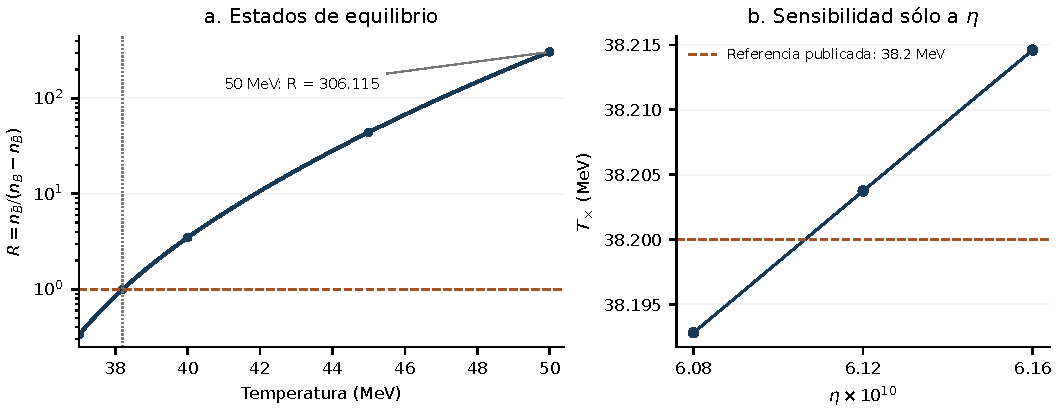
\includegraphics[width=.98\textwidth]{figures/final_cross_es.pdf}
\caption{Cociente de antibariones respecto del exceso neto para PDG2025. Izquierda: secuencia de estados de equilibrio entre 37 y 50 MeV; los puntos indican evaluaciones propias y la línea horizontal, $R=1$. Derecha: temperatura de cruce obtenida para el valor central y los extremos de la incertidumbre de entrada de $\eta$; la línea entre puntos es una guía visual. La referencia de 38.2 MeV procede de Yang y Rafelski (2022); no se le asigna una incertidumbre no publicada.}
\label{fig:cross}
\end{figure*}

Los tres inventarios dieron cruces cercanos (Tabla~\ref{tab:crosscatalogs}). Entre PDG2014 y PDG2025, la amplitud numérica fue $0.000142$ MeV. Al variar sólo $\eta$ en $(6.12\pm0.04)\times10^{-10}$, el cruce PDG2025 abarcó 38.192814--38.214598 MeV y $R(50)$ abarcó 304.1237--308.1319. Esta sensibilidad de entrada fue mayor que la diferencia con el valor bibliográfico redondeado y que la amplitud de estos tres catálogos.

\begin{table}[t]\centering\small
\caption{Sensibilidad al inventario con la misma entrada cosmológica. Los decimales adicionales documentan el cálculo, no su exactitud física.}
\label{tab:crosscatalogs}
\begin{tabular}{lrr}\toprule
Lista & $T_\times$ (MeV) & $R(50\ {\rm MeV})$\\\midrule
PDG2014 & 38.203596 & 306.128980\\
PDG2020 & 38.203739 & 306.114776\\
PDG2025 & 38.203739 & 306.114688\\
\bottomrule\end{tabular}
\end{table}


\subsection{Cantidades en una misma región comóvil}
Las conversiones cosmológicas dieron $n_{\gamma0}=410.7268$ cm$^{-3}$ y $n_{b0}=(2.514\pm0.017)\times10^{-7}$ cm$^{-3}$, compatibles con la densidad bariónica media compilada por \citet{Groom2025}. Esta compatibilidad verifica la conversión de entradas compartidas, sin constituir una predicción independiente del residuo.

La región comóvil que corresponde hoy a 1 m$^3$ contiene en promedio 0.251365 unidades de número bariónico neto. A 50 MeV, el cálculo asignó a esa misma región aproximadamente 77.1978 bariones y 76.9465 antibariones, con suma 154.1443 y la misma diferencia 0.251365. En el cruce, las cantidades fueron 0.502730 y 0.251365, respectivamente. Son cantidades medias normalizadas al volumen actual, no las densidades de un m$^3$ físico del plasma temprano ni eventos acumulados de regeneración.

La composición primordial equivalente dio $n_{H0}^{\rm prim}=(1.898\pm0.015)\times10^{-7}$, $n_{{}^4He,0}^{\rm prim}=(1.540\pm0.021)\times10^{-8}$ y $n_{D0}^{\rm prim}=(4.760\pm0.066)\times10^{-12}$ cm$^{-3}$. Estas cantidades convierten abundancias nucleares externas a la densidad media actual; el HRG de 50 MeV no predijo la producción posterior de H, He o D. La comparación común se establece a través del número bariónico neto.

\subsection{Verificación numérica e información recuperable}
Los 24 controles se completaron satisfactoriamente. La diferencia relativa máxima al pasar de 96 a 192 términos fue $4.44\times10^{-16}$ y el error relativo máximo de cierre de $Y_{\Delta B}$, $1.25\times10^{-14}$. Las integrales independientes de nucleones coincidieron con las sumas dentro de $1.23\times10^{-15}$. Estas cifras cuantifican consistencia computacional, sin medir la exactitud física del modelo.

La prueba de rango confirmó que el residuo solo aporta una ecuación para dos poblaciones: añadir el mismo rendimiento a bariones y antibariones deja intacto $Y_{\Delta B}$. El equilibrio, el inventario y la temperatura aportaron la relación adicional que permitió reconstruir las poblaciones de la Tabla~\ref{tab:states}. No se obtuvo una selección única de la historia de producción y aniquilación a partir de las abundancias presentes.

\section{Discusión}
El objetivo se respondió afirmativamente para estados de equilibrio condicionados: las propiedades de las especies de partícula y el exceso bariónico cosmológico permitieron inferir cantidades separadas de bariones y antibariones a una temperatura bibliográfica especificada. El resultado central a 50 MeV cuantifica una población casi simétrica y un exceso pequeño, con 306.1 antibariones por unidad neta. Al enfriarse los estados calculados, el mismo cociente alcanzó la unidad cerca del hito de 38.2 MeV publicado por \citet{Yang2022}. La sucesión coincide con el comportamiento general descrito por \citet{Satarov2013}.

La coincidencia debe interpretarse dentro de las condiciones compartidas. Ambos enfoques relacionan equilibrio hadrónico con información cosmológica sobre el exceso por entropía. Aquí se utilizaron inventarios fijados y una implementación independiente de las sumas térmicas; no se reprodujo la evolución cinética de Satarov et al. ni se realizó una réplica completa del modelo de Yang y Rafelski. Estos últimos imponen neutralidad eléctrica y de extrañeza, mientras nuestro cálculo mantuvo $\mu_Q=\mu_S=0$. Además, sus entradas cosmológicas no son idénticas. Por ello, la diferencia con 38.2 MeV no puede atribuirse exclusivamente al catálogo, ni presentarse como una prueba independiente de observaciones tempranas.

La condición química simplificada tiene un efecto verificable: sumando las cargas de las especies de partícula exportadas, a 50 MeV se obtuvo un número de carga neta igual a aproximadamente $0.4901\,\Delta n_B$ y un número de extrañeza neta de $-0.03253\,\Delta n_B$. Los leptones con potencial químico nulo no compensaron esa carga. El estado reconstruido es, por tanto, una aproximación térmica declarada; completar la reconstrucción cosmológica física requeriría resolver simultáneamente los balances de carga, extrañeza y sector leptónico. Esta limitación subsiste aunque el cruce numérico redondee a la referencia publicada.

Las cantidades comóviles aclaran la relación con el presente. El exceso se conserva bajo los supuestos adoptados, mientras el total de bariones y antibariones de equilibrio disminuye. Comparar directamente un cm$^3$ temprano y uno actual mezclaría el cambio de población con la dilución por expansión. La normalización por entropía permite comparar una misma región y declarar cantidades medias sin introducir un volumen cosmológico global no documentado. Las abundancias de H, He y D sirven como referencias nucleares externas de otra etapa; su cálculo histórico exige una red de nucleosíntesis posterior.

La reconstrucción histórica completa requiere tasas de producción inversa, aniquilación y decaimiento, junto con expansión y condiciones iniciales. En un esquema homogéneo, una ecuación del tipo
\begin{align}
\frac{dn_{\bar B}}{dt}+3Hn_{\bar B}
&=\langle\sigma v\rangle\bigl(n_B^{\rm eq}n_{\bar B}^{\rm eq}
-n_Bn_{\bar B}\bigr)\label{eq:kinetic}
\end{align}
introduce información que una tabla de equilibrio no contiene; $H$ es la tasa de expansión y $\langle\sigma v\rangle$ el promedio térmico del producto de la sección eficaz y la velocidad relativa. No se integró esa ecuación en este trabajo. Por ello no se determinaron el primer evento, el final cinético ni el número acumulado de partículas regeneradas.

La aportación del trabajo es una referencia cuantitativa reproducible que conecta entradas actuales con inventarios tempranos bajo supuestos explícitos, identifica la información recuperable y muestra el alcance del contraste publicado. No se establece una nueva observación, una explicación del origen de la asimetría o un mecanismo físico nuevo. La convergencia numérica y la sensibilidad a una entrada no sustituyen la evaluación de neutralidad, interacciones, anchos de resonancia y validez del equilibrio.

\section{Conclusiones}
Los cálculos permitieron reconstruir poblaciones de equilibrio condicionadas a masas de reposo, inventario HRG, temperatura y exceso cosmológico. A la referencia bibliográfica de 50 MeV se obtuvieron $2.7261\times10^{30}$ bariones y $2.7172\times10^{30}$ antibariones por cm$^3$, con exceso de $8.8765\times10^{27}$ cm$^{-3}$. Coexistieron 306.1147 antibariones por unidad del exceso neto; los nucleones y sus antipartículas aportaron 95.2176\% del total.

El criterio $n_{\bar B}=n_B-n_{\bar B}$ se alcanzó a 38.203739 MeV con PDG2025 y redondeó al hito publicado de 38.2 MeV. La variación de $\eta$ por sí sola desplazó el cruce a 38.192814--38.214598 MeV. El contraste aporta consistencia de modelos de equilibrio con condiciones relacionadas, sin determinar una incertidumbre física total.

La abundancia actual sola no identificó una población inicial única ni un historial de aniquilación. La aproximación $\mu_Q=\mu_S=0$ dejó carga y extrañeza netas distintas de cero. Estos límites delimitan la conclusión: se logró una reconstrucción térmica cuantitativa y reproducible, y una reconstrucción cosmológica completa requiere balances químicos y evolución cinética adicionales.

\section*{Disponibilidad de datos y código}
El paquete adjunto incluye fuentes de los manuscritos, figuras por idioma, catálogos fijados y licencia, 18 estados agregados para tres listas, 1329 registros por especie de partícula para PDG2025, curva del cruce, sensibilidad a $\eta$, 24 controles numéricos y guía de ejecución en Windows. Las conversiones cosmológicas y el análisis previo se conservan como antecedentes identificados. El cálculo se ejecutó en Python con una implementación independiente; se utilizaron los datos de Thermal-FIST, sin ejecutar su programa C++.

\section*{Asistencia en la preparación}
Se utilizó asistencia de inteligencia artificial para preparar redacción, código, figuras y maquetación. Los cálculos y controles descritos se ejecutaron y sus salidas se conservaron. El lanzador PowerShell se revisó estáticamente; no se ejecutó en Windows. La interpretación científica y la decisión de publicación corresponden al autor.



\onecolumn
\begin{multicols}{2}
\begin{thebibliography}{99}\small
\setlength{\itemsep}{2pt}
\bibitem[Fields et al.(2025)]{Fields2025}
Fields, B. D., Molaro, P., \& Sarkar, S. (2025).
Big Bang nucleosynthesis. In \emph{Review of Particle Physics: 2025 update}.
\href{https://pdg.lbl.gov/2025/reviews/rpp2025-rev-bbang-nucleosynthesis.pdf}{PDG review}.

\bibitem[Fixsen(2009)]{Fixsen2009}
Fixsen, D. J. (2009).
The temperature of the cosmic microwave background.
\emph{The Astrophysical Journal, 707}(2), 916--920.
\doi{10.1088/0004-637X/707/2/916}.

\bibitem[Groom and Scott(2025)]{Groom2025}
Groom, D. E., \& Scott, D. (2025).
Astrophysical constants and parameters. In \emph{Review of Particle Physics: 2025 update}, Table 2.1.
\href{https://pdg.lbl.gov/2025/reviews/rpp2025-rev-astrophysical-constants.pdf}{PDG constants table}.

\bibitem[Particle Data Group(2025)]{PDG2025}
Particle Data Group. (2025).
Muon properties. In \emph{Review of Particle Physics: 2025 update}.
\href{https://pdg.lbl.gov/2025/listings/rpp2025-list-muon.pdf}{PDG muon listing}.

\bibitem[Robinson and Zyla(2025)]{Robinson2025}
Robinson, D., \& Zyla, P. A. (2025).
Physical constants. In \emph{Review of Particle Physics: 2025 update}, Table 1.1.
\href{https://pdg.lbl.gov/2025/reviews/rpp2025-rev-phys-constants.pdf}{PDG physical constants}.

\bibitem[Satarov et al.(2013)]{Satarov2013}
Satarov, L. M., Mishustin, I. N., \& Greiner, W. (2013).
Evolution of antibaryon abundances in the early Universe and in heavy-ion collisions.
\emph{Physical Review C, 88}, 024908.
\doi{10.1103/PhysRevC.88.024908}.

\bibitem[Vovchenko and Stoecker(2019)]{Vovchenko2019}
Vovchenko, V., \& Stoecker, H. (2019).
Thermal-FIST: A package for heavy-ion collisions and hadronic equation of state.
\emph{Computer Physics Communications, 244}, 295--310.
\doi{10.1016/j.cpc.2019.06.024}.

\bibitem[Vovchenko and Stoecker(2026)]{TFLists2026}
Vovchenko, V., \& Stoecker, H. (2026).
\emph{Thermal-FIST: PDG2014, PDG2020, and PDG2025 light-and-strange particle lists}
[Data files, repository snapshot \texttt{4086191e9522}].
\href{https://github.com/vlvovch/Thermal-FIST/tree/4086191e952285cd572ba2bbbefb2fdc55401c9b/input/list}{GitHub repository snapshot}.

\bibitem[Yang and Rafelski(2022)]{Yang2022}
Yang, C. T., \& Rafelski, J. (2022).
Cosmological strangeness abundance.
\emph{Physics Letters B, 827}, 136944.
\doi{10.1016/j.physletb.2022.136944}.

\end{thebibliography}

\end{multicols}
\end{document}
